% Please add the following required packages to your document preamble:
% \usepackage{multirow}
% \begin{table*}[]
% \vspace{4pt}
% \resizebox{\textwidth}{!}{
% \centering
% \begin{tabular}{c|c|c|c|c|c|c|c|}
%   \cline{2-8}
%   &
%   \multicolumn{3}{c|}{\textbf{Task Time [seconds]}} &
%   \multicolumn{3}{c|}{\textbf{Number of Actions}} &
%   \multicolumn{1}{c|}{\textbf{Success Rate}} \\ \hline
%   \multicolumn{1}{|c|}{\textbf{Planner}} &
%   \textbf{S4} &
%   \textbf{S5} &
%   \textbf{S6} &
%   \textbf{S4} &
%   \textbf{S5} &
%   \textbf{S6} &
%   \textbf{S4 - S6} \\ \hline
% \multicolumn{1}{|c|}{PokeRRT*} &
%   \textbf{69.58 (26.15)} &
%   \textbf{127.45 (57.80)} &
%   182.03 (122.77) &
%   \textbf{5.27 (2.00)} &
%   \textbf{5.12 (1.05)} &
%   \textbf{6.11 (1.91)} &
%   \textbf{0.9 (0.3)} \\ \hline
% \multicolumn{1}{|c|}{PokeRRT} &
%   83.55 (29.59) &
%   148.55 (86.23) &
%   \textbf{157.03 (94.41)} &
%   6.20 (1.60) &
%   6.67 (1.56) &
%   6.88 (2.15) &
%   \textbf{0.9 (0.3)}\\ \hline
% \multicolumn{1}{|c|}{Two-Level Push Planner} &
%   120.21 (47.09) &
%   N/A &
%   N/A &
%   6.00 (1.26) &
%   N/A &
%   N/A &
%   0.33 (0.47) \\ \hline\hline
% \multicolumn{1}{|c|}{Pick-and-Place} &
%   N/A &
%   20.31 (3.21) &
%   N/A &
%   N/A &
%   1.00 (0.00) &
%   N/A &
%   0.27 (0.44) \\ \hline
% \end{tabular}
% }
% \caption{Real-world task times, number of actions in executed path, and success rates are presented in this table. Results are averaged across 10 trials. Pushing has the highest success rate and fastest task times. PokeRRT* generates plans with the fewest number of actions.\vspace{-14pt}}
% \label{tab:eval-real}
% \end{table*}

\begin{table*}[]
\vspace{4pt}
\centering\small
\resizebox{0.95\textwidth}{!}{
\centering
\begin{tabular}{|c|c|c|c|c|c|}
  \hline
   \textbf{Planner} & & PokeRRT* & PokeRRT & Two-Level Push Planner & Pick-and-Place \\
   \hline
  \multirow{3}{*}{\textbf{Task Time [seconds]}} & \textbf{S4} & \textbf{69.58 (26.15)} & 83.55 (29.59) & 120.21 (47.09) & N/A \\ \cline{2-6}
  & \textbf{S5} & \textbf{127.45 (57.80)} & 148.55 (86.23) & N/A & 20.31 (3.21) \\ \cline{2-6}
  & \textbf{S6} & 182.03 (122.77) & \textbf{157.03 (94.41)} & N/A & N/A \\ \hline
  \multirow{3}{*}{\textbf{Number of Actions}} & \textbf{S4} & \textbf{5.27 (2.00)} & 6.20 (1.60) & 6.00 (1.26) & N/A \\ \cline{2-6}
  & \textbf{S5} & 5.12 (1.05) & 6.67 (1.56) & N/A & \textbf{1.00 (0.00)} \\ \cline{2-6}
  & \textbf{S6} & \textbf{6.11 (1.91)} & 6.88 (2.15) & N/A & N/A \\ \hline
%   \multirow{3}{*}{\textbf{Initial Planning Time}} & \textbf{S4} & 4.64 (1.70) & 7.19 (7.26) & 19.10 (8.66) & N/A \\ \cline{2-6} 
%   & \textbf{S5} & 18.95 (12.41) & 29.97 (31.22) & N/A & N/A \\ \cline{2-6}
%   & \textbf{S6} & 15.38 (14.35) & 22.91 (34.66) & N/A & N/A \\ \hline
  \multirow{3}{*}{\textbf{Number of Replans}} & \textbf{S4} & 3.45 (1.67) & 4.2 (1.6) & \textbf{2.80 (1.54)} & N/A \\ \cline{2-6} 
  & \textbf{S5} & \textbf{3.38 (1.32)} & 4.11 (1.37) & N/A & N/A \\ \cline{2-6}
  & \textbf{S6} & \textbf{4.22 (1.81)} & 4.38 (1.49) & N/A & N/A \\ \hline
%   \multirow{3}{*}{\textbf{Replanning Times}} & \textbf{S4} & 4.75 (1.72) & 3.4 (2.01) & 10.04 (4.56) & N/A \\ \cline{2-6} 
%   & \textbf{S5} & 16.42 (9.89) & 11.58 (10.79) & N/A & N/A \\ \cline{2-6}
%   & \textbf{S6} & 22.56 (19.65) & 11.28 (10.32) & N/A & N/A \\ \hline
%   \multirow{3}{*}{\textbf{Execution Time}} & \textbf{S4} & 9.21 (0.5) & 9.53 (0.86) & 11.16 (0.46) & N/A \\ \cline{2-6} 
%   & \textbf{S5} & 9.47 (0.48) & 9.11 (0.28) & N/A & N/A \\ \cline{2-6}
%   & \textbf{S6} & 8.84 (0.23) & 10.20 (1.70) & N/A & N/A \\ \hline
  \textbf{Success Rate} & \textbf{S4 - S6} & \textbf{0.9 (0.3)} & \textbf{0.9 (0.3)} & 0.33 (0.47) & 0.27 (0.44)\\ \hline
\end{tabular}
}
\caption{Real-world task times, number of actions in executed path, and success rates are presented in this table. Results are averaged across 10 trials. Pushing has the highest success rate and fastest task times. PokeRRT* generates plans with the fewest number of actions.\vspace{-12pt}}
\label{tab:eval-real}
\end{table*}

\begin{figure}
\vspace{4pt}
  \centering
    \hspace{-7pt}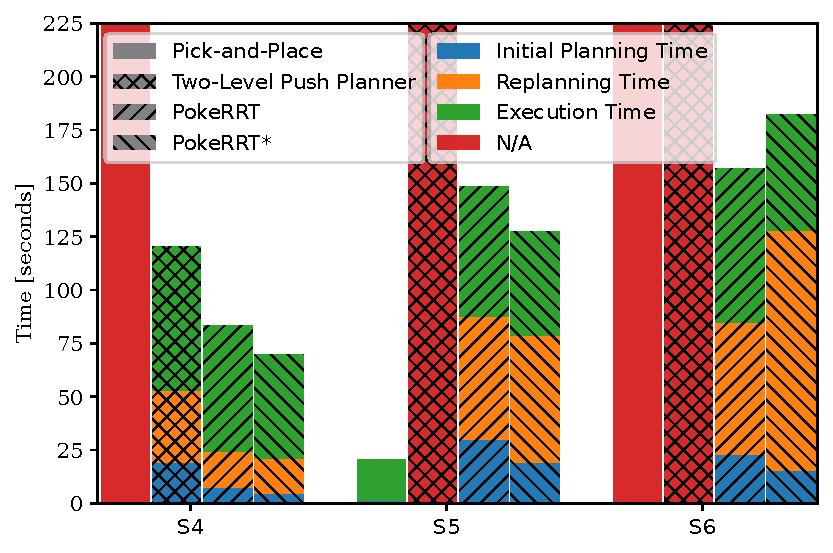
\includegraphics[width=\linewidth]{figures/plot.pdf}
%   \vspace{-12pt}
  \caption{A breakdown of task time as the sum of initial planning, replanning, and execution times is presented for various planners in the real-world. A single bar indicates total task time. Long red bars indicate cases where tasks cannot be solved. Overall, poke planning demonstrates lower execution and replanning times than push planning. \vspace{-10pt}}\label{fig:plot}
\end{figure}
